% translate_docs: ./manuals/preconditioning_manual.tex @ 2a57ad48e16e3e1949a46e871e394e3d2231476f
\documentclass[superscriptaddress,onecolumn,floatfix]{revtex4-2}

\usepackage{graphicx}
\usepackage{epsfig}
\usepackage{color}
\usepackage{amssymb}
\usepackage{amsmath}
\usepackage{array}
\usepackage[loose]{units}
\usepackage{hyperref}
\usepackage{cleveref}
\usepackage{tasks}
\usepackage[caption=false]{subfig}
\usepackage[german]{babel}
\usepackage{letltxmacro}

\LetLtxMacro{\ORIGselectlanguage}{\selectlanguage}
\makeatletter
\DeclareRobustCommand{\selectlanguage}[1]{%
    \@ifundefined{alias@\string#1}
      {\ORIGselectlanguage{#1}}
      {\begingroup\edef\x{\endgroup
         \noexpand\ORIGselectlanguage{\@nameuse{alias@#1}}}\x}%
}
\newcommand{\definelanguagealias}[2]{%
  \@namedef{alias@#1}{#2}%
}
\makeatother

\definelanguagealias{de}{german}


\begin{document}
\selectlanguage{de}

\begin{abstract}
  Dieses Handbuch behandelt die grundlegende Verwendung und häufig gestellte Fragen zum manuellen Vorkonditionierungsset.
\end{abstract}
\title{Handbuch für das Vorbehandlungsset}
\author{Electroniq Buttons Boutique}
\email{support@electroniqbuttons.com}
\date{\today}

\maketitle


\section{Welche Autos können das nutzen?} \label{sect:eligibility}
Das Kit ist für die meisten Ioniq 5-Modelle (2021–2024), Ioniq 6-Modelle (2022–2025) und EV6-Modelle (2022–2024) geeignet. Wir haben es an Ioniq 5-Modellen aus drei verschiedenen Märkten sowie an einem Ioniq 6 und einem EV6 getestet. \href{mailto:requests@electroniqbuttons.com}{Kontaktieren Sie uns} Falls Sie das Set in einem anderen Fahrzeug verwenden möchten: Es funktioniert nur mit einer Batterieheizung. Um dies zu überprüfen, suchen Sie bitte im Menü „EV“ nach dem „Batteriekonditionierungsmodus“. $\to$ EV-Einstellungen (siehe Abb. \ref{subfig:menus:EVsettings}) auf dem Headunit (zentraler Bildschirm) Ihres Autos (siehe Abb. \ref{subfig:menus:batt_cond}).
\begin{figure}[h]
  \subfloat[]{\label{subfig:menus:EVsettings}
  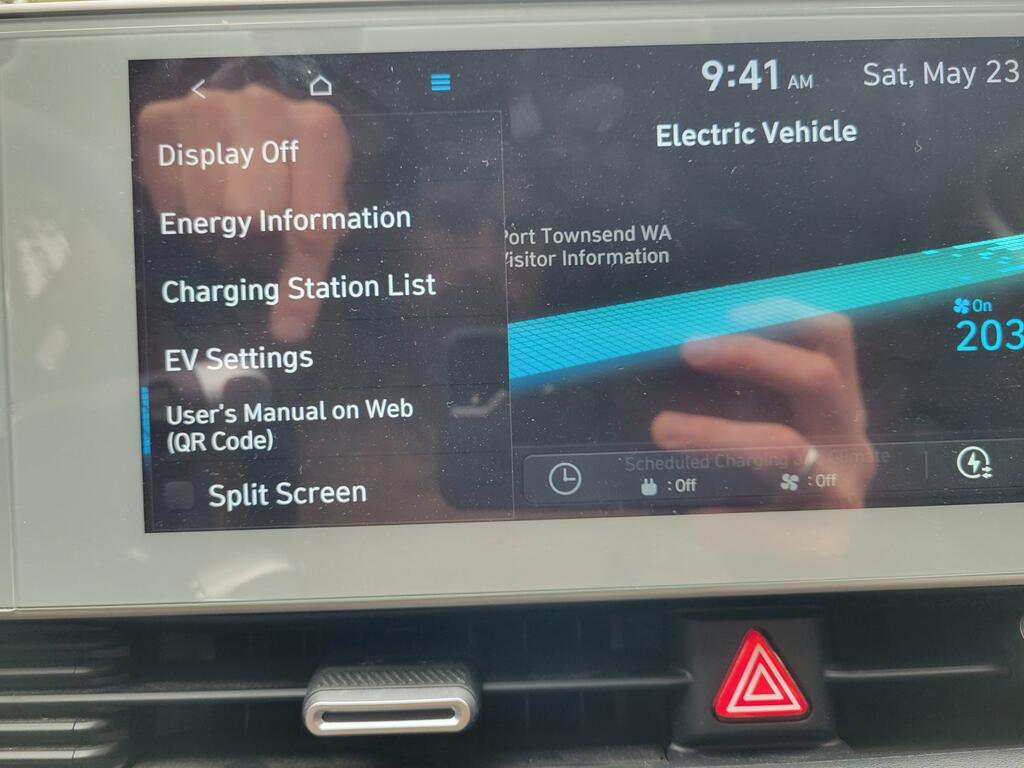
\includegraphics[height=1.95in]{photos/EV_settings.jpg} }
  \subfloat[]{\label{subfig:menus:batt_cond}
  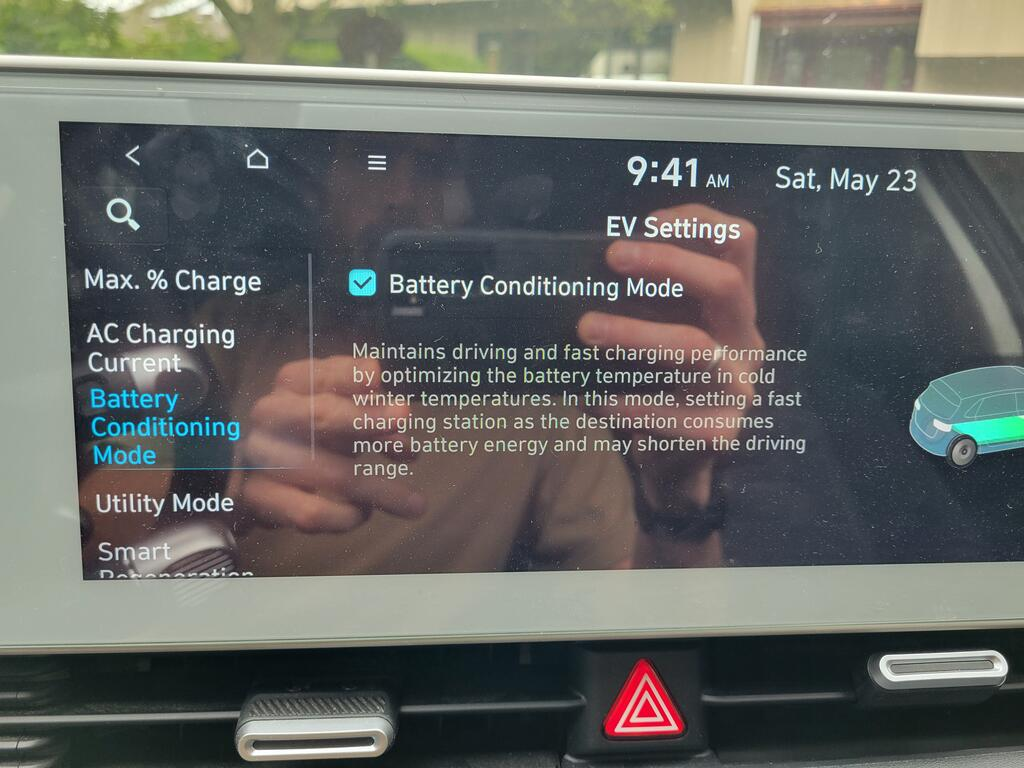
\includegraphics[height=1.95in]{photos/battery_conditioning_mode.jpg} }
   \caption{(a) So finden Sie das Menü für die EV-Einstellungen: Tippen Sie auf dem Hauptbildschirm auf das Symbol „EV“; tippen Sie anschließend im daraufhin erscheinenden Menü auf der linken Seite auf „EV-Einstellungen“. (b) Bildschirm „Batteriekonditionierungsmodus“. \label{fig:menus}}
\end{figure}

Falls Ihr Fahrzeug diesen Bildschirm nicht besitzt, sollten Sie dieses Set nicht kaufen. Bitte wenden Sie sich an einen Händler oder an erfahrene Fahrzeughalter in Ihrem Land, um zu klären, ob die Nachrüstung dieser Funktion in Ihrem Fahrzeug mit zusätzlichen Schritten möglich ist. Für die USA, Kanada oder Norwegen kontaktieren Sie uns bitte unter [Kontaktinformationen einfügen]. \href{mailto:support@electroniqbuttons.com}{support@electroniqbuttons.com} Gerne helfen wir Ihnen bei der Beurteilung anhand einiger Informationen zu Ihrem Auto.

Wenn anstelle des in Abbildung 1 dargestellten „Batteriekonditionierungsmodus“ \ref{subfig:menus:batt_cond}Wenn Ihr Fahrzeug den „Wintermodus“ aktiviert hat, benötigt es lediglich ein Firmware-Update von einem Händler. Suchen Sie die entsprechende technische Serviceinformation für Ihr Land zu diesem Update und wenden Sie sich an Ihren nächstgelegenen autorisierten Händler. Nach Abschluss dieses Schritts und Bestätigung, dass der Menüpunkt „Batteriekonditionierungsmodus“ den „Wintermodus“ ersetzt hat, können Sie dieses Kit erwerben.

\section{Grundausstattung}
Beginnen Sie mit dem \href{https://github.com/tylerharvey/Ioniq5_CAN/blob/main/guides/}{Installationsanleitungen}. Sehen \href{https://meatpihq.github.io/wican-fw/config/wifi}{WiCAN-Dokumente} Für die grundlegende WiCAN-Einrichtung. Dies ist für die Aktivierung der Vorkonditionierung nicht erforderlich, es wird jedoch dringend empfohlen, zumindest das Standard-WLAN-Passwort aus Sicherheitsgründen zu ändern.  

\section{Benutzeroberfläche}
Wir entwickeln die Benutzeroberfläche rasant weiter, schauen Sie also regelmäßig hier vorbei!

Um das manuelle Vorkonditionierungsverhalten zu konfigurieren, verbinden Sie sich mit dem WiCAN-WLAN und besuchen Sie die WiCAN-Konfigurationsseite unter \href{http://192.168.80.1}{http://192.168.80.1}Die dritte Registerkarte mit der Bezeichnung „Schaltflächen“ ist in Abbildung 1 dargestellt. \ref{subfig:ui:buttons} ermöglicht die Konfiguration der manuellen Vorkonditionierungstaste und aller anderen benutzerdefinierten Tasten, die später hinzugefügt werden.

\begin{figure}[h]
  \subfloat[]{\label{subfig:ui:buttons}
  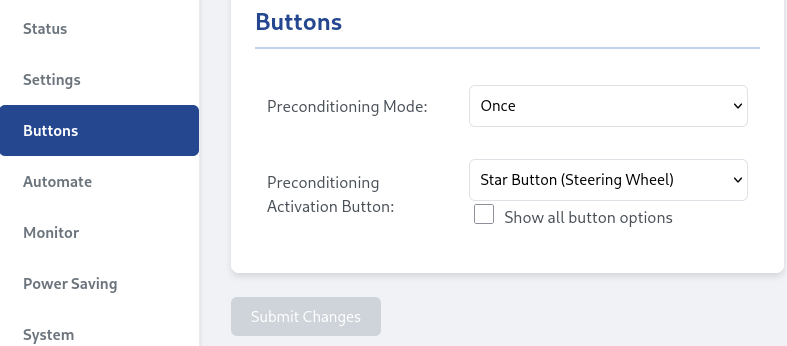
\includegraphics[height=1.95in]{photos/ui_2026-07-04.png} }  \\
   \caption{Screenshot der Seite „Schaltflächen“ in der WiCAN-HTTP-Konfiguration.}
\end{figure}

Die erste Option, der „Vorkonditionierungsmodus“, befindet sich derzeit in der Entwicklung und kann nur einmalig aktiviert werden. Nach einem einzigen Vorkonditionierungszyklus wird die Vorkonditionierung beendet. Wir arbeiten an den Modi „Kontinuierlich“ und „Persistent“, die es dem Batteriemanagementsystem (BMS) ermöglichen, die Batterie automatisch wieder aufzuheizen, wenn die Temperatur sinkt – entweder bis zum Abstellen des Fahrzeugs („Kontinuierlich“) oder sogar während des Ein- und Ausschaltens des Fahrzeugs („Persistent“).

Die zweite Option ermöglicht die Auswahl einer Taste zur Zuweisung der Vorkonditionierung. Weitere Optionen stehen mit dem angepassten WiCAN im Man-in-the-Middle-Modus zur Verfügung. Standardmäßig werden 5 Optionen angezeigt:
\begin{enumerate}
  \item Deaktiviert
  \item Sterntaste (Lenkrad) -- Standard
  \item Stern-Schaltfläche (Klimaleiste)
  \item Tuner Press (Klimabar)
  \item Volumenpresse (Klimabar)
\end{enumerate}
Bei der Option „Deaktiviert“ wird durch keine Taste die Vorkonditionierung ausgelöst. Dies kann beim Werkstattbesuch in einer Vertragswerkstatt von Vorteil sein, um Verwirrung bei den Servicetechnikern zu vermeiden. Die „Drücken“-Optionen beziehen sich auf das Drücken der Tasten, nicht auf Drehen oder Drücken nach oben oder unten. Sollte keine dieser Optionen funktionieren, können Sie das Kontrollkästchen „Alle Tastenoptionen anzeigen“ aktivieren, um weitere Optionen freizuschalten.
\begin{tasks}(2)
  \task Modus (Lenkrad)
  \task Sprechen (Lenkrad)
  \task Anruf (Lenkrad)
  \task Lautstärkeregler (Lenkrad)
  \task Lautstärke erhöhen (Lenkrad)
  \task Lautstärke verringern (Lenkrad)
  \task Nach oben springen (Lenkrad)
  \task Nach unten springen (Lenkrad)
  \task OK (Lenkrad)
  \task Karte (Klimabalken)
  \task Navigation (Klimaleiste)
  \task Medien (Klimabalken)
  \task Tuner Up (Klimabar)
  \task Tuner Down (Klimaleiste)
\end{tasks}
Wählen Sie den für Sie passenden Button! Wir hoffen, bald auch physische Buttons anbieten zu können.

Um die Vorkonditionierung manuell zu aktivieren, drücken Sie einfach die gewünschte Aktivierungstaste. Sofort erscheint ein Countdown in Metern/Yards im Kombiinstrument, der die Entfernungsanzeige überlagert. Wenn der Tempomat eingeschaltet ist, wird die Entfernungsanzeige teilweise verdeckt. Navigieren Sie mit der Seitentaste am Lenkrad zur Seite mit den Navigationsanweisungen im Kombiinstrument. Die Vorkonditionierung startet, sobald der Countdown Null erreicht hat. Sollte der Countdown zurückgesetzt werden, ist ein unerwartetes Problem aufgetreten und der Vorgang wird wiederholt. 

Wenn die Vorkonditionierung aktiviert wird, erscheint das Standard-Popup mit der Meldung „Batterievorkonditionierung für optimales DC-Laden aktiviert“ (siehe Abbildung). \ref{subfig:precon:popup}Außerdem wird über dem Batteriesymbol in der unteren linken Ecke des Kombiinstruments ein Schneeflocken- oder rotes Spulensymbol angezeigt (siehe Abbildung). \ref{subfig:precon:coil}.

\begin{figure}[h]
  \subfloat[]{\label{subfig:precon:popup}
  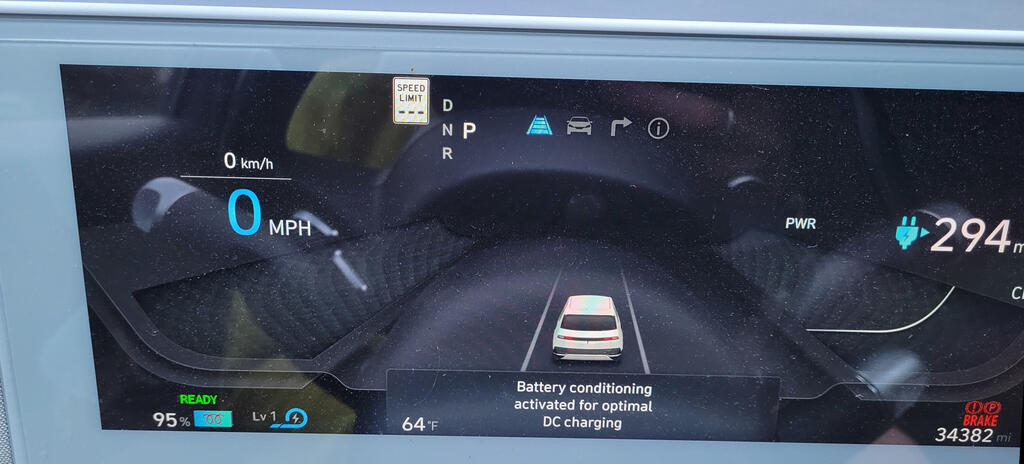
\includegraphics[height=1.95in]{photos/precon_active.jpg} }  \\
  \subfloat[]{\label{subfig:precon:coil}
  
\includegraphics[height=1in]{photos/coil_on_battery.jpg} }
   \caption{(a) Screenshot des Pop-ups, das die erfolgreiche Aktivierung der Batterievorkonditionierung anzeigt. (b) Beispiel-Screenshot des Spulensymbols, das über dem Batteriesymbol in der unteren linken Ecke des Kombiinstruments liegt. \label{fig:precon}}
\end{figure}

Falls die Vorkonditionierung nicht aktiviert wird, überprüfen Sie, ob die integrierten Aktivierungsbedingungen erfüllt sind:
\begin{enumerate}
  \item Die Batterietemperatur muss unter folgendem Wert liegen: $\unit[21]{C}$/$\unit[70]{F}$
  \item Der Wert des Ladezustands muss höher sein als $\unit[20]{\%}$
  \item Der Bildschirm „Batteriekonditionierungsmodus“ ist im Menü „EV-Einstellungen“ vorhanden (siehe Abschnitt 1). \ref{sect:eligibility})
\end{enumerate}
Leider handelt es sich hierbei um Einschränkungen, die in der Firmware der Batteriemanagementeinheit oder der Hardware des Fahrzeugs verankert sind und die wir mit diesem Kit nicht ändern können.

\section{Stromverbrauch}
Dieses Set wird über das 12-V-Bordnetz Ihres Autos betrieben, das heißt, es kann Strom von der 12-V-Batterie Ihres Autos beziehen. Dazu sollten einige Punkte besprochen werden:
\begin{enumerate}
  \item Wie viel Strom verbraucht es?
  \item Wird es die 12V-Batterie zerstören?
  \item MITM vs. parallel
\end{enumerate}

\subsection{Wie viel Strom verbraucht es?}

Wir haben den Stromverbrauch mehrerer Mikrocontroller in verschiedenen Zuständen bei ausgeschaltetem Fahrzeug (12,7 V) gemessen. Die WiCAN-Tests im Normalbetrieb wurden ohne HTTP-Anfragen und ohne BLE-Verbindung über CarScanner oder ähnliches durchgeführt. Diese Tests erfolgten am wählbaren CAN-Kabelbaum, über den unseres Wissens derzeit keine OBD-Anfragen möglich sind. Daher verbrauchten die Mikrocontroller mit Standard-OBD-Funktionalität (WiCAN, vLinker MC+) wahrscheinlich weniger Strom als beim aktiven Abfragen von OBD-Parametern über den normalen OBD-Anschluss. 

\subsubsection{WiCAN Originalversion 4.20\_eb0.1.1-beta19}
\begin{enumerate}
  \item{Normale Verwendung:} 30 mA
  \item{Verwendung von HTTP-Seiten:} bis zu 34 mA
  \item{Startvorgang:} bis zu 36 mA
  \item{CAN-Überwachung:} bis zu 38 mA
  \item{Schlafen:} $<$1 mA
\end{enumerate}

\subsubsection{WiCAN Custom, erste Version, läuft mit Version 4.20\_eb0.1.1-beta19}
\begin{enumerate}
  \item{Normale MITM-Nutzung:} 40 mA
  \item{Normale parallele Nutzung:} 34 mA
  \item{Startvorgang:} bis zu 48 mA
\end{enumerate}

\subsubsection{WiCAN Pro läuft mit Version 4.50}
\begin{enumerate}
  \item{Normale Verwendung:} 50 mA
\end{enumerate}

\subsubsection{Komma-weißer Panda rennt als letzter Animatronic\_Panda Build}
\begin{enumerate}
  \item{Normale Verwendung:} 32 mA
\end{enumerate}

\subsubsection{vLinker MC+}
\begin{enumerate}
  \item{Normaler Gebrauch (ohne Verbindung):} 15-18 mA
  \item{CarScanner ist über BLE verbunden:} 20-25 mA, Stromspitzen bis zu 60 mA
\end{enumerate}

\subsection{Wird es die 12V-Batterie zerstören?}

WiCAN verfügt über einen Energiesparmodus, den sogenannten Schlafmodus, in dem nahezu alle Funktionen heruntergefahren werden und der Stromverbrauch minimal ist. Dieser Modus ist normalerweise so konfiguriert, dass er sich anhand der 12-V-Spannung Ihres Fahrzeugs einschaltet. Wenn Sie Bedenken hinsichtlich Ihrer 12-V-Spannung haben, empfehlen wir Ihnen, diese Funktion zu aktivieren. Sie finden sie in der WiCAN-Benutzeroberfläche unter [Pfad einfügen]. \href{http://192.168.80.1}{http://192.168.80.1} im Tab „Energiesparen“. Weitere Informationen finden Sie hier: \href{https://meatpihq.github.io/wican-fw/config/sleep-mode}{https://meatpihq.github.io/wican-fw/config/sleep-mode}Wir arbeiten aktiv daran, diese Funktion von spannungsbasiert auf CAN-basiert (d. h. auf das Signal „Fahrzeug aus“ achten) umzustellen. 

Mit einer neuen 60-Ah-12-V-Batterie würde der typische Stromverbrauch des angepassten WiCAN von 40 mA über 7 Tage betragen. $40 \unit[\mathrm{mA}] * 24 \unit[\mathrm{hours/day}] * 7 \unit[\mathrm{days}] = 6.7 Ah$, was ungefähr 10 entspricht.\% of the 12V state of charge. Unlocked and off, a 2022 Canadian Preferred AWD Ioniq 5 with no aftermarket loads draws about 1.75 A (1750 mA). After ECUs quiet down 5 minutes after locking the car, the draw is still 0.75 A (750 mA). (The car has a further "sleep" mode after 7 days of inactivity; this draw hasn't been measured here.) So, a customized WiCAN in MITM mode and not in sleep mode increases draw over the first 7 days of inactivity by 5\%.

\subsection{MITM vs. Parallel}
Wenn der Kabelbaum des Vorkonditionierungskits im MITM-Modus ist und Ihr WiCAN-System in den Schlafmodus wechselt, werden Anfragen an die Hyundai/Kia-App nicht verarbeitet. Langfristig ist geplant, einen Teilschlafmodus einzuführen, der die CAN-Weiterleitung ermöglicht, WLAN jedoch deaktiviert. Wir empfehlen, Ihr WiCAN-System im Schlafmodus mit einer sehr niedrigen Spannung, z. B. 12,3 V, zu betreiben, wenn der Kabelbaum im MITM-Modus ist und Sie Anfragen an die Hyundai/Kia-App nutzen möchten. 

\section{Häufig gestellte Fragen}
\begin{enumerate}
  \item[Q:] Wie installiere ich es?
  \item[A:] Siehe die \href{https://github.com/tylerharvey/Ioniq5_CAN/blob/main/guides/}{Installationsanleitungen}Falls Ihnen das zu kompliziert erscheint, fragen Sie doch einfach einen Teenager in Ihrer Nähe oder einen Car-Audio-Händler um Hilfe!
  \item[Q:] Warum funktionieren meine Rückfahrkamera, die Auto-App oder andere Funktionen des zentralen Bildschirms nach der Installation nicht?
  \item[A:] Überprüfen Sie die \href{https://github.com/tylerharvey/Ioniq5_CAN/blob/main/guides/harnesses/head_unit_MITM/MITM_harness_modes.pdf}{Leitfaden zu den Gurtmodi}Wenn Sie ein originales WiCAN-System verwenden oder kein Gerät an den OBD-Anschluss angeschlossen ist, muss der Kabelbaum im Parallelmodus betrieben werden. Bei einem kundenspezifischen WiCAN-System muss der Kabelbaum im MITM-Modus betrieben werden.
  \item[Q:] Wird mein Auto dadurch leichter gestohlen?
  \item[A:] Unwahrscheinlich, aber die Installation ist aus verschiedenen Gründen, unter anderem aus Sicherheitsgründen, so konzipiert, dass sie schwer zu erkennen ist. Wir empfehlen Ihnen dringend, Ihr WiCAN-Passwort zu ändern. 
  \item[Q:] Wird dadurch meine Garantie ungültig?
  \item[A:] Informieren Sie sich über die Garantie- und Verbraucherschutzgesetze Ihres Landes. In den USA bietet der Magnusson-Moss Warranty Act einen starken Verbraucherschutz. Drohungen von Autoherstellern, dass Zubehörteile aus dem Zubehörhandel die Garantie ungültig machen, sind in vielen Fällen vor Gericht nicht haltbar. (Dies ist keine Rechtsberatung.) Gleichzeitig ist die Fehlerdiagnose durch einen Kfz-Techniker oft schwierig. Wir empfehlen daher dringend, alle Zubehörteile und Nachrüstteile zu entfernen, die die Diagnose erschweren könnten. Wenn Sie beispielsweise Probleme mit dem Autoradio oder dem USB-Anschluss haben, ist es ratsam, diese Teile vor dem Werkstattbesuch auszubauen, um Komplikationen bei der Diagnose zu vermeiden. 
  \item[Q:] Welche Konfiguration des Kits wird für die Durchführung einer grundlegenden Wartung meines Autos in der Vertragswerkstatt empfohlen?
  \item[A:] Wir empfehlen Ihnen, Ihr WiCAN-Gerät vom Stromnetz zu trennen und sicherzustellen, dass Ihr Kabelbaum angeschlossen ist. \href{https://github.com/tylerharvey/Ioniq5_CAN/blob/main/guides/harnesses/head_unit_MITM/MITM_harness_modes.pdf}{Parallelmodus}.
  \item[Q:] Was, wenn ich das selbst bauen möchte?
  \item[A:] Mach es! Alles, was wir getan haben, ist \href{https://github.com/tylerharvey/Ioniq5_CAN}{Open-Source}Sie können den Schaltplan gerne verwenden, um selbst etwas zu bauen. Die Stecker sind auf AliExpress erhältlich. Wenn Sie jedoch einen Beitrag zum öffentlichen Wissen in Form eines Pull Requests an die Community leisten, … \href{https://github.com/dragz/egmpdbc}{DBC-Datei} Oder es gibt andere Möglichkeiten: Es gibt Rabatte, die die Nettokosten auf ein mit DIY-Angeboten konkurrenzfähiges Niveau senken, und das bei deutlich geringerem Arbeitsaufwand.
  \item[Q:] Warum kann das nicht ein Software-Update sein?
  \item[A:] Das könnte sein. Wir haben Vermutungen, warum Hyundai/Kia dies nicht in ein Navigationsupdate aufgenommen hat. Wenn Sie wissen, wie… \href{https://discord.gg/zyrngQ5qQ}{Hacke dein Autoradio} und die CAN-Schnittstellenfunktionen gefunden haben, können Sie diese gerne hinzufügen. \href{https://www.reddit.com/r/KiaEV6/comments/1jdd56u/comment/mid9xie/}{eine manuelle Vorkonditionierungstaste an Ihrem Autoradio}Die Verbreitung von manipulierter Firmware ist derzeit jedoch nicht möglich, weshalb ein nachträgliches „Update“ nur schwer flächendeckend verfügbar zu machen wäre.
  \item[Q:] Kann ich das auf meinem Comma-Gerät implementieren?
  \item[A:] Wir haben dies getestet und glauben nicht, dass es funktioniert. Anscheinend werden keine Vorkonditionierungsnachrichten von den CAN-Bussen A oder E, an denen das Comma-Modul angeschlossen ist, an die CAN-Busse M oder G weitergeleitet, an denen das BMU-Modul angeschlossen ist.
  \item[Q:] Wird das meine ICCU zerstören?
  \item[A:] NEIN.
  \item[Q:] Kann ich die integrierte Navigation während der Verwendung dieses Kits nutzen?
  \item[A:] In der Beta-Version ist dies nicht möglich. Dies wird mit dem angepassten WiCAN behoben.
  \item[Q:] Wird ein Navigationsupdate meine Fähigkeit, das Kit zu nutzen, beeinträchtigen?
  \item[A:] Es ist höchst unwahrscheinlich, da das Kit nicht auf die Kommunikation mit dem Steuergerät angewiesen ist. Ein Update des Batteriemanagementsystems wäre möglich (beispielsweise das Update, das die Vorkonditionierung bei frühen Ioniq 5-Modellen nachträglich aktivierte), aber wir gehen davon aus, dass solche Updates von Vertragshändlern durchgeführt werden müssen. Eine hundertprozentige Garantie können wir jedoch nicht geben.\% certainty that a navigation update will not affect the functionality of the kit. In the off chance that this does happen, let us know and we will do our best to update logic to restore manual preconditioning functionality.
  \item[Q:] Warum der Countdown? Warum kann die Vorkonditionierung nicht einfach direkt nach dem Drücken der Taste beginnen?
  \item[A:] Das Batteriemanagementsystem (das Steuergerät im Akku, das das BMS enthält) verfügt über eine integrierte 60-Sekunden-Wartezeit nach der ersten Vorkonditionierungsanforderung. Wird die Anforderung vor Ablauf dieser 60 Sekunden abgebrochen, startet die Vorkonditionierung nicht. Daher haben wir versucht, diese 60-Sekunden-Wartezeit für den Benutzer deutlich sichtbar und verständlich zu gestalten.
  \item[Q:] Würdest du mir einen neuen Knopf bauen?
  \item[A:] Vielleicht! Schreiben Sie uns eine E-Mail an \href{mailto:requests@electroniqbuttons.com}{requests@electronicbuttons.com} mit Ihren Anfragen.
  \item[Q:] Ihr Geschäft heißt „Electroniq Buttons Boutique“. Wo befinden sich die physischen Knöpfe?
  \item[A:] Wir arbeiten daran, physische Tasten anzubieten. Roy hat einen getesteten Prototyp, der in seinem Video gezeigt wird. \href{https://github.com/dragz/ironiq}{Ironiq} Repository.
\end{enumerate}
% \begin{figure}[h]
%   \subfloat[]{\label{subfig:overview:harness}
%   \includegraphics[height=1.95in]{photos/whole_harness.jpg} }
%   \subfloat[]{\label{subfig:overview:shunt_cap_labeled}
%   \includegraphics[height=1.95in]{photos/labeled_connectors_MITM_harness.jpg} }
%    \caption{(a) Man-in-the-middle harness. (b) Overview of connectors showing shunt cap. \label{fig:overview}}
% \end{figure}
\appendix 
\bibliographystyle{apsrev4-1}
\bibliography{stemh_model}{}
\end{document}
